

  % begin the content of the document
\sloppy  % this to relax whitespacing in favour of straight margins


% title on top of the document
\maintitle{Werner Mostert}{July 29,1994}{Last update on \today}

\nobreakvspace{0.3em}  % add some page break averse vertical spacing

\noindent\href{mailto:werner.dot.mostert1.at.gmail.dot.com}{werner.mostert1\mbox{}@\mbox{}gmail.com}\sbull
\textsmaller{+}27.713618606\sbull
\href{https://za.linkedin.com/pub/werner-mostert/99/341/258}{https://za.linkedin.com/pub/werner-mostert/99/341/258}
\\
2203 The Gables\sbull
1138 Prospect Street\sbull
Hatfield\sbull
Pretoria\\

\spacedhrule{0.9em}{-0.4em}  % a horizontal line with some vertical spacing before and after
\begin{center}
\roottitle{Summary}  % a root section title
\end{center}


\vspace{-1.3em}  % some vertical spacing
\begin{multicols}{3}% open a multicolumn environment

\noindent \fbox{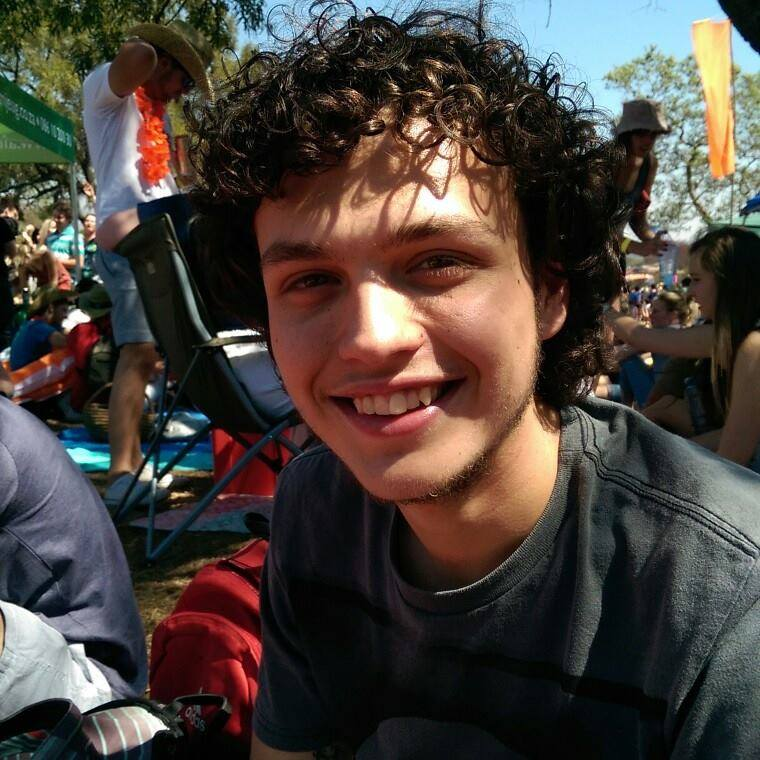
\includegraphics[width=\linewidth]{werner}}\\I am a very driven person with very clear goals in terms of my career as well as my personal life. I believe in honesty above all else and making a valuable contribution towards society. In my opinion, one of the greatest injustices that can be done by man, is refusing to pass on what one has learnt and experienced, for without this happening there can be no progress. My dream is to be remembered for the feats that I had accomplished in my lifetime. I am extremely passionate about technology, specifically software development, which is the reason why I chose to study Computer Science at a tertiary level. I am particularly fond of new challenges that test my abilities allowing for growth, self-improvement and the improvement of others. My family and friends are an extremely important factor in my life and I would see them proud of the man that I am, and want to be. 

\end{multicols}

\spacedhrule{0em}{-0.4em}

\roottitle{Experience}

\headedsection
  {\href{http://www.bbd.co.za}{Barone, Budge \& Dominick (Pty) Ltd}}
  {\textsc{Houghton Estate, Johannesburg}} {%
  \headedsubsection
    {Bursar}{Jan\apo15 -- present}
    {\bodytext{BBD implements and maintains complex business systems. A customer with a requirement for custom software, which must fit into their business, and must meet the business goals approaches BBD with the goal in mind of obtaining a software solution thereof.\\}}
    }
    
\headedsection
  {\href{http://www.bbd.co.za}{University of Pretoria, Computer Science Department}}
  {\textsc{Hatfield, Pretoria}} {%
  \headedsubsection
    {Teaching Assistant}{Jul\apo14 -- present}
    {\bodytext{As a teaching assistant for Data Structures and Algorithms, Netcentric Computer Systems and Software Modelling it is expected of one to have a good understanding of design patterns, general algorithm implementations and data structures in the Computer Science field as well as knowledge of web development and other networking related software development.\\}}
    }
    
\headedsection  % sets the header for the section and includes any subsections
  {\href{http://www.dvt.co.za}{Dynamic Visual Technologies}}
  {\textsc{Hyde Park, Johannesburg}} {%
  \headedsubsection
    {Junior Software Developer}
    {Nov \apo14 -- Jan\apo15}
    {\bodytext{DVT is a software development and related services business. They build, implement and support software, and  provide those services that ensure business concepts are clear, that practical needs are met, and that software is written to specifications. \\}}
}
    
\spacedhrule{-0.2em}{-0.4em}


\roottitle{Technical Skills}

\inlineheadsection  % special section that has an inline header with a 'hanging' paragraph
  {Technical expertise:}
  {Software design and implementation. Big fan of Agile methodologies. I regularly utilise Java/\nsp \CPP, yet flirts regularly with C\#.  Proper knowledge of web technologies:\ \acr{HTML+CSS}, \acr{XML},  \acr{REST}, \acr{SOAP} and JavaScript (including WebGL). Elementary knowledge of Artificial Intelligence related methods, such as optimisation problems.}

\vspace{0.5em}
\inlineheadsection
  {Natural languages:}
  {Afrikaans \emph{(mother tongue)}, English \emph{(full professional proficiency)}, French \emph{(elementary proficiency)}.}


\spacedhrule{1.6em}{-0.4em}

\roottitle{Interests}
\inlineheadsection
  {Non-exhaustive:}
  {Online gaming, running, music, reading, travel, foreign cultures, most things French related, cooking, open source movements, software development.}

  
\spacedhrule{1.6em}{-0.4em}  
  
\roottitle{Non - Technical Strengths}

\inlineheadsection
  {Social skills:}
  {I believe myself to be a rather "likeable" person, meaning I am very seldom found to be antagonistic towards others. I am a people person. I enjoy meeting and spending time with new and interesting people.}
  
\inlineheadsection
  {Professional skills:}
  {In a professional working environment I strive to be a very punctual, concise and informed individual. My approach towards professionalism relies on the concepts of honesty, determination, perseverance and most of all proper communication.}
  
\spacedhrule{1.6em}{-0.4em}  
  
\roottitle{Why DVT Drive Stats?}

\inlineheadsection
  {Because:}
  {I am very interested in mobile development, particularly for Android devices. I feel this project is very applicable to modern day life and can actually make a difference in people's lives. As a result of my previous experience with DVT, I will always jump to the opportunity to engage with the people and company.}